\DocumentMetadata{pdfversion=1.7,pdfstandard=A-3a,tagging=on,lang=zh-cn}
\documentclass[zihao=5,UTF8,fontset=windows]{ctexart}

\usepackage{amsmath}
\usepackage{mathtools}
\usepackage{unicode-math}
\usepackage{geometry}
\usepackage{float}
\usepackage{tikz}
\usepackage[pdfusetitle]{hyperref}
\usepackage{fancyhdr}
\usepackage{graphics}
\usepackage{booktabs}
\usepackage{tcolorbox}
\usepackage{tabularx}

\geometry{hmargin=1in,vmargin=1in,a4paper}

% \makeatletter
\hypersetup{
	colorlinks,
	linkcolor=blue,
	% pdfencoding=auto,
	% pdftitle={\@title},
	% pdfauthor={\@author},
	% pdfcreator=LaTeX
}
% \makeatother

\tcbset{
	before upper={\parindent2em}
}

\usetikzlibrary{graphdrawing,graphs,arrows.meta}
\usegdlibrary{layered}

\author{石成玉}
\title{读基于超声波振动的肥箱抗粘减阻特性分析与装置设计}
\date{2025年9月24日}

\begin{document}

\maketitle

\tableofcontents

\section{研究背景}

\begin{enumerate}
	\item \textbf{水果产业矛盾}：中国是水果生产大国，但不是水果生产强国。
	\item \textbf{没有充分利用中国的自然资源优势}：水果产业优质发展不仅需要充足的营养，还需要好的果园管理技术，尤其是\textbf{土壤养分管理}
	\item \textbf{土壤有机质含量低}：土壤有机质对果树优质生长发挥了重大的作用。施用有机肥可改善土壤有机质含量
\end{enumerate}

\section{问题和思考}

\subsection{为什么要开展有机肥施肥？}

\begin{enumerate}
	\item \textbf{水果产业矛盾：}中国是水果生产大国，但不是水果生产强国。
	\item \textbf{没有充分利用中国的自然资源优势：}水果产业优质发展不仅需要充足的营养，还需要好的果园管理技术，尤其是\textbf{土壤养分管理}
	\item \textbf{土壤有机质含量低：}土壤有机质对果树优质生长发挥了重大的作用。施用有机肥可改善土壤有机质含量
	\item 团队研制过一种果园施肥机，但是在施有机肥时会因为\textbf{肥料与箱底粘附}增加施肥阻力，甚至造成堵塞
	\item \textbf{减粘技术：}比如改变表面形貌减粘脱附技术、机械减粘脱附技术、加热减粘脱附技术等，都有其局限性
	\item \textbf{振动减粘：}低频振动能减轻触土部件的阻力；\textbf{高频低幅振动（超声波）}在金属加工中有较多应用，能\textbf{有效降低}加工时的阻力。
	\item \textbf{目的：}将超声波振动带到施肥机中
\end{enumerate}

\subsection{有机肥施肥装备存在问题是什么？}

施肥机施肥过程中易出现肥料与箱底粘附，导致排肥装置工作阻力增大，最终造成有机肥堵塞影响施肥机正常施肥等问题。

\begin{enumerate}
	\item \textbf{可遥控的履带式自走式果园开沟施肥机：}
	
    \begin{itemize}
		\item 未考虑肥料肥箱内流动性较差；
		\item 排肥装置容易发生堵塞
	\end{itemize}
	
	\item \textbf{分层施肥机：}
	
	\begin{itemize}
		\item 两侧土量过多导致前进阻力较大
	\end{itemize}
	
	\item \textbf{果园开沟施肥机}：
	
	\begin{itemize}
		\item 肥料粘附堵塞
	\end{itemize}
\end{enumerate}

\subsection{有机肥施肥存在的问题会带来哪些影响？}

肥料与肥箱底部黏附的问题会导致：

\begin{enumerate}
	\item \textbf{施肥阻力大：}

	\begin{itemize}
		\item 增加施肥时消耗的能量；
		\item 增加施肥机部分零件承受的载荷导致其过早失效；
	\end{itemize}
	
	\item \textbf{肥箱堵塞：}
	
	\begin{itemize}
		\item 使施肥中断，降低施肥效率；
		\item 频繁维修，增加工人劳动量；
		\item 施肥不均匀；
	\end{itemize}
\end{enumerate}

\section{论文试验中存在哪些问题}

\subsection{关于有机肥与钢板的摩擦系数的测量问题}

\begin{tcolorbox}
	\textbf{2.2 超声振动对有机肥料摩擦角影响试验材料与方法}

	\begin{figure}[H]
		\centering
		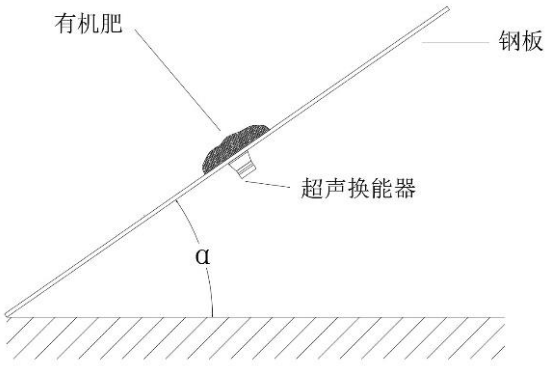
\includegraphics[width=0.8\textwidth,alt=有机肥摩擦角试验原理.png]{../assets/有机肥摩擦角试验原理.png}
		\caption{试验装置示意图}
		\label{fig:有机肥摩擦角试验原理示意图}
	\end{figure}

	\begin{flushright}
		——曹欢-\emph{基于超声波振动的肥箱抗粘减阻特性分析与装置设计}
	\end{flushright}	
\end{tcolorbox}

\begin{enumerate}
	\item 有机肥颗粒是松散材料，在倾斜钢板的过程中，应该测量哪一时刻的倾斜角度？肉眼观察有机肥开始滚动的时刻是否误差过大？
	\item 测量开启超声波换能器后的摩擦角时，换能器从启动到相对稳定存在一过程。测量时，如果先开启换能器至其状态相对稳定，有机肥与钢板的接触状态就会发生较大改变，是否存在较大误差？改进方案：首先倾斜钢板至换能器未开启时，有机肥发生移动的临界点，再开启换能器。若开启换能器后有机肥发生移动则减小倾斜角度，否则增加倾斜角度。利用枚举法或者二分法测得开启换能器时的有机肥与钢板的摩擦角度。
\end{enumerate}

\subsection{超声振动频率对有机肥摩擦角的影响}

\begin{tcolorbox}
		\begin{flushleft}
			\textbf{2.3.1 超声振动频率对有机肥摩擦角的影响}
		\end{flushleft}
		
		由图2-12可知，超声振动频率对有机肥的摩擦角有不同影响。随着超声波频率增加，有机肥的摩擦角先减小后增大，减摩率先上升后下降。当超声频率为28kHz时，超声减摩效果最佳。这主要是因为超声振动会导致接触面摩擦副发生高频、小振幅的法向振动。随着频率的增加，振动使得有机肥和钢板之间的有效接触面积减小，从而使摩擦角的减小程度增大。随着频率的进一步增加，钢板质点的振动频率也增加。由于施加在换能器上的功率相同，频率越高，换能器转化为振幅的能量就越低。{\color{red} 因此，换能器端面的振幅降低，有机肥颗粒与钢板接触面积开始增大，进而减摩效果降低。}因此，40kHz超声振动的减摩效果较差。

		\begin{flushright}
			——曹欢-\emph{基于超声波振动的肥箱抗粘减阻特性分析与装置设计}
		\end{flushright}

\end{tcolorbox}

	振幅降低为什么会导致有机肥颗粒与钢板的接触面积增大？振幅改变是否影响有机肥颗粒与钢板的接触时间？

\section{智能控制方面如果你来做有哪些可以优化的地方？}

\begin{enumerate}
	\item 是否可以考虑使用不断变化的频率？
	\item 可以根据阻力的大小动态调节换能器的功率。
	\item 可以在出肥孔增加流量传感器以保证出肥速率稳定，使施肥均匀。
	\item 可以增加堵塞处理机构，使得堵塞时能自行恢复。
\end{enumerate}

\subsection{其他问题}

\subsubsection{超声振动施加方式·纵向振动施加方式}

\begin{table}[H]
	\centering
	\begin{tabular}{cc}
		\toprule
		变量 & \\
		\midrule
		有机肥在钢板上的恒定滑动速度 & $V_0$ \\
		摩擦副的振幅 & $\alpha$ \\
		角速度 & $\omega$ \\
		\bottomrule
	\end{tabular}
\end{table}

振动函数

\[V_{(t)}=\alpha \omega \sin ( \omega t) \tag{2-1}\label{振动函数}\]

整个循环阶段的平均摩擦力

\[F = \frac{F_0}{T}(4t_s) \tag{2-2}\label{average_force}\]

其中

\[T=\frac{2\pi}{\omega} \tag{2-3}\label{周期}\]

又公式$\eqref{average_force}$和$\eqref{周期}$得：

\[t_s=\frac{FT}{4F_0}=\frac{F}{4F_0}\times\frac{2\pi}{\omega}=\frac{F\pi}{2F_0\omega} \tag{2-4}\]

\section{想法}

\begin{enumerate}
	\item 给换能器添加梯台形状的匀波板。
	\item 使用多个不同频率或者功率的换能器交替使用以实现频率和功率可变。
	\item 叠加使用不同频率的换能器来改变波形。
\end{enumerate}

\end{document}